% !TEX encoding = UTF-8 Unicode
%%%%%%%%%%%%%%%%%%%%%%%%%%%%%%%%%%%%%%%%%
% Beamer Presentation
% LaTeX Template
% Version 1.0 (10/11/12)
%
% This template has been downloaded from:
% http://www.LaTeXTemplates.com
%
% License:
% CC BY-NC-SA 3.0 (http://creativecommons.org/licenses/by-nc-sa/3.0/)
%
%%%%%%%%%%%%%%%%%%%%%%%%%%%%%%%%%%%%%%%%%

%----------------------------------------------------------------------------------------
%	PACKAGES AND THEMES
%----------------------------------------------------------------------------------------
\documentclass{beamer}

\usepackage[utf8]{inputenc}
\usepackage[finnish]{babel}

\mode<presentation> {

% The Beamer class comes with a number of default slide themes
% which change the colors and layouts of slides. Below this is a list
% of all the themes, uncomment each in turn to see what they look like.

%\usetheme{default}
%\usetheme{AnnArbor}
%\usetheme{Antibes}
%\usetheme{Bergen}
%\usetheme{Berkeley}
%\usetheme{Berlin}
%\usetheme{Boadilla}
%\usetheme{CambridgeUS}
%\usetheme{Copenhagen}
%\usetheme{Darmstadt}
%\usetheme{Dresden}
%\usetheme{Frankfurt}
%\usetheme{Goettingen}
%\usetheme{Hannover}
%\usetheme{Ilmenau}
%\usetheme{JuanLesPins}
%\usetheme{Luebeck}
\usetheme{Madrid}
%\usetheme{Malmoe}
%\usetheme{Marburg}
%\usetheme{Montpellier}
%\usetheme{PaloAlto}
%\usetheme{Pittsburgh}
%\usetheme{Rochester}
%\usetheme{Singapore}
%\usetheme{Szeged}
%\usetheme{Warsaw}

% As well as themes, the Beamer class has a number of color themes
% for any slide theme. Uncomment each of these in turn to see how it
% changes the colors of your current slide theme.

%\usecolortheme{albatross}
%\usecolortheme{beaver}
%\usecolortheme{beetle}
%\usecolortheme{crane}
%\usecolortheme{dolphin}
%\usecolortheme{dove}
%\usecolortheme{fly}
%\usecolortheme{lily}
%\usecolortheme{orchid}
%\usecolortheme{rose}
%\usecolortheme{seagull}
\usecolortheme{seahorse}
%\usecolortheme{whale}
%\usecolortheme{wolverine}

%\setbeamertemplate{footline} % To remove the footer line in all slides uncomment this line
\setbeamertemplate{footline}[page number] % To replace the footer line in all slides with a simple slide count uncomment this line

%\setbeamertemplate{navigation symbols}{} % To remove the navigation symbols from the bottom of all slides uncomment this line
}

\usepackage{graphicx} % Allows including images
\usepackage{booktabs} % Allows the use of \toprule, \midrule and \bottomrule in tables
\usepackage{textcomp} % \textrightarrow

\DeclareUnicodeCharacter{00A0}{~}

%----------------------------------------------------------------------------------------
%	TITLE PAGE
%----------------------------------------------------------------------------------------

\title[Internet of Shit]{Internet of Shit} % The short title appears at the bottom of every slide, the full title is only on the title page

\author{Mikko Tuohimaa} % Your name
\date{20.5.2017} % Date, can be changed to a custom date

\begin{document}

\begin{frame}
\titlepage % Print the title page as the first slide
\end{frame}

\section{Lupaus}

\begin{frame}
\frametitle{IoT:n lupaus} % Table of contents slide, comment this block out to remove it
\begin{block}{}
Kaikki liitetään Internetiin
\end{block}
\begin{itemize}
	\item Valtava muutos elämän ja teollisuuden joka osa-alueella
	\item Lähes rajattomasti uutta bisnespotentiaalia
	\item Vientiä parisuhdemarkkinoilla
	\item ...
\end{itemize}
\end{frame}

\begin{frame}
\frametitle{IoT:n lupaus}
\begin{itemize}
\item Automatisointi
\item Etäkäyttö
\item Big Data
\item Analytiikka
\item Ennakoiva huolto
\item Uudet bisnesmallit
\end{itemize}
\end{frame}

\section{Todellisuus}

\begin{frame}
\frametitle{IoT:n todellisuus}
\begin{figure}
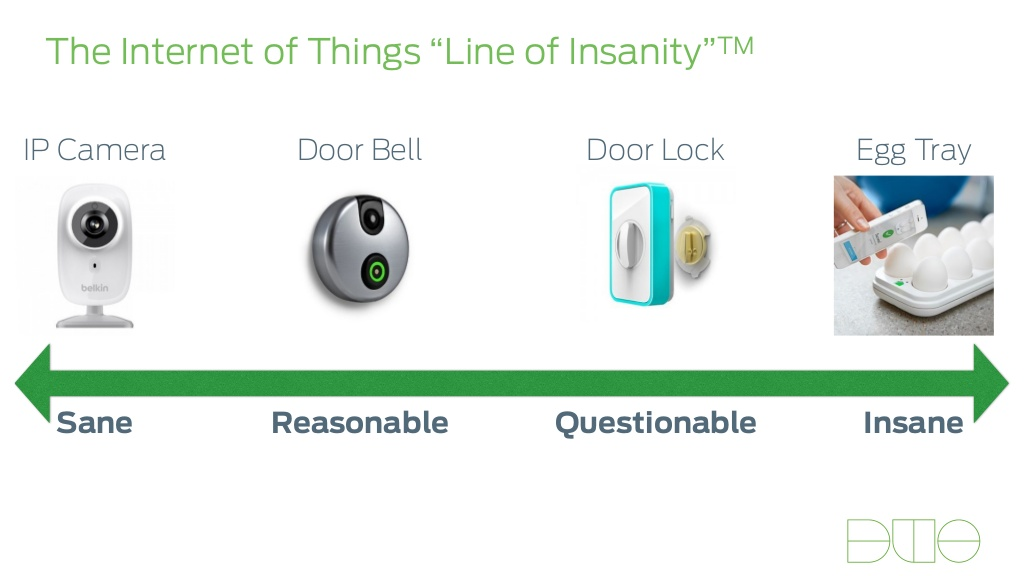
\includegraphics[width=\linewidth]{line-of-insanity}
\end{figure}
\end{frame}

\begin{frame}
\frametitle{Ratkaiseeko IoT jonkin oikean ongelman?}
\begin{figure}
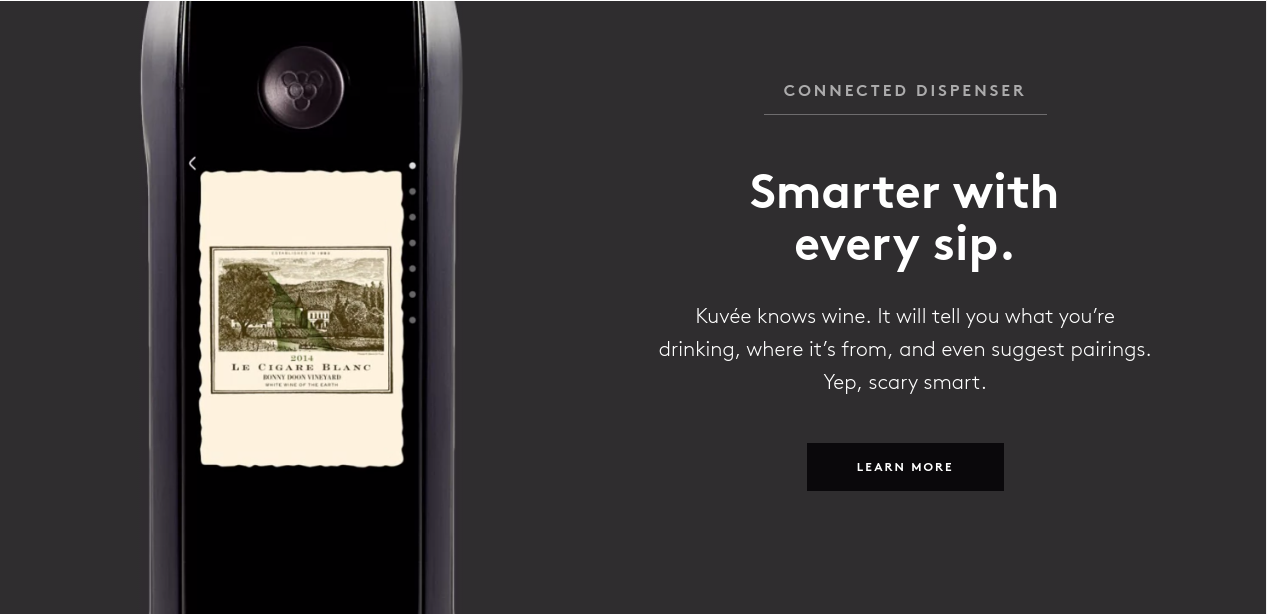
\includegraphics[width=\linewidth]{wine-bottle}
\end{figure}
\end{frame}


\begin{frame}
\frametitle{Ratkaiseeko IoT jonkin oikean ongelman?}
\begin{figure}
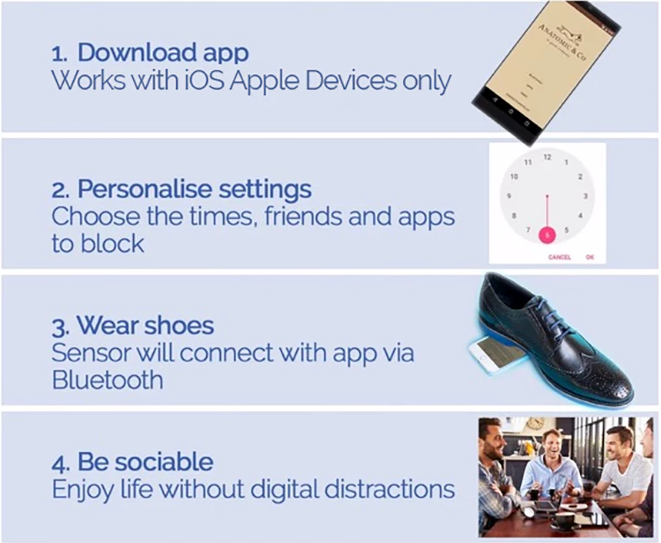
\includegraphics[width=0.8\linewidth]{shoes}
\end{figure}
\end{frame}

\begin{frame}
\frametitle{Ratkaiseeko IoT jonkin oikean ongelman?}
\begin{figure}
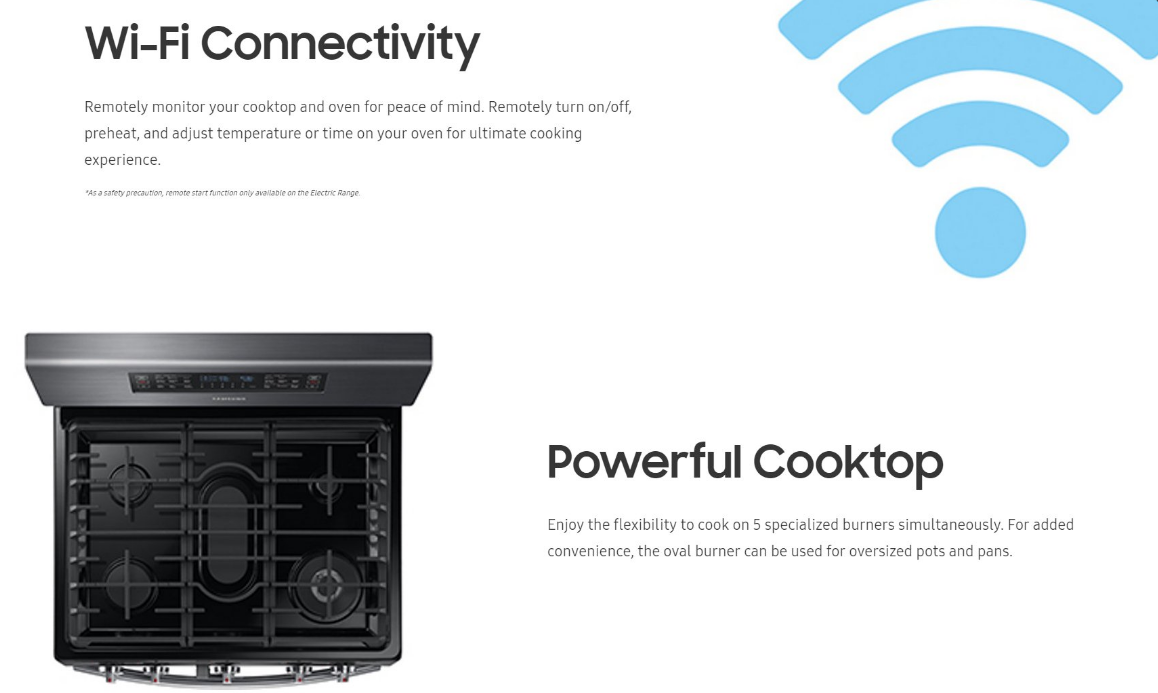
\includegraphics[width=\linewidth]{uuni}
\end{figure}
\end{frame}

\section{Suorat ongelmat}

\begin{frame}
\frametitle{Mitä jos...}
\begin{figure}

\includegraphics[width=0.6\linewidth]{stop}
\end{figure}
\end{frame}

\begin{frame}
\frametitle{Mitä jos... yhteys bugaa}
\begin{figure}

\includegraphics[width=\linewidth]{juicer}
\end{figure}
\end{frame}

\begin{frame}
\frametitle{Mitä jos... yhteys bugaa}
\begin{figure}

\includegraphics[width=\linewidth]{hybrid-watch}
\end{figure}
\end{frame}

\begin{frame}
\frametitle{Mitä jos... yhteys bugaa}
\begin{figure}

\includegraphics[width=\linewidth]{uuni2}
\end{figure}
\end{frame}

\begin{frame}
\frametitle{Mitä jos... softa pitää päivittää}
\begin{figure}
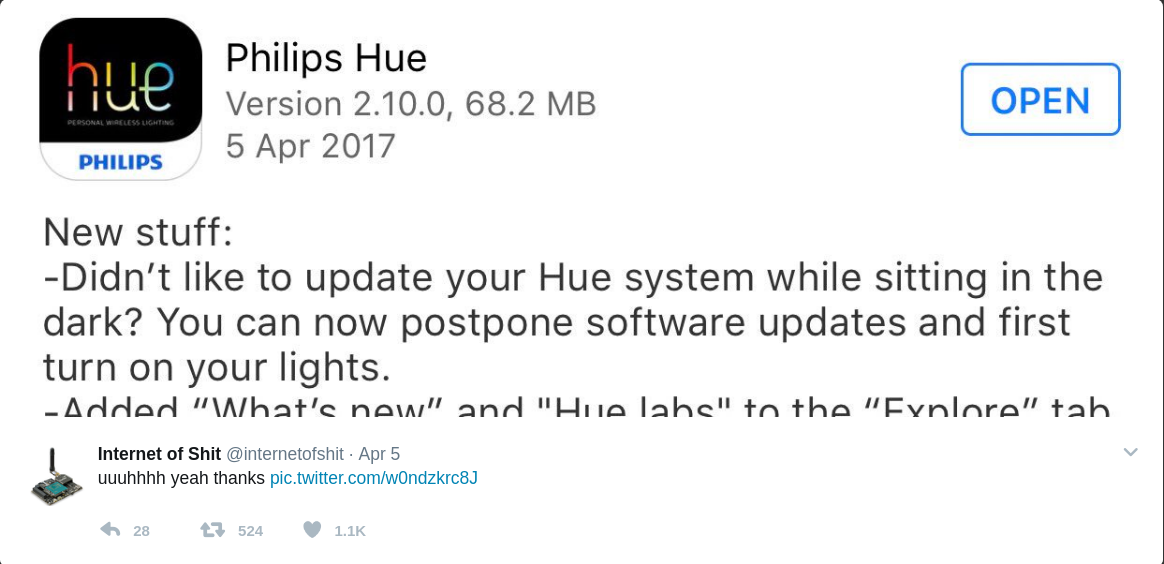
\includegraphics[width=\linewidth]{hue-update-in-the-dark}
\end{figure}
\end{frame}

\begin{frame}
\frametitle{Mitä jos... tuki loppuu}
\begin{figure}
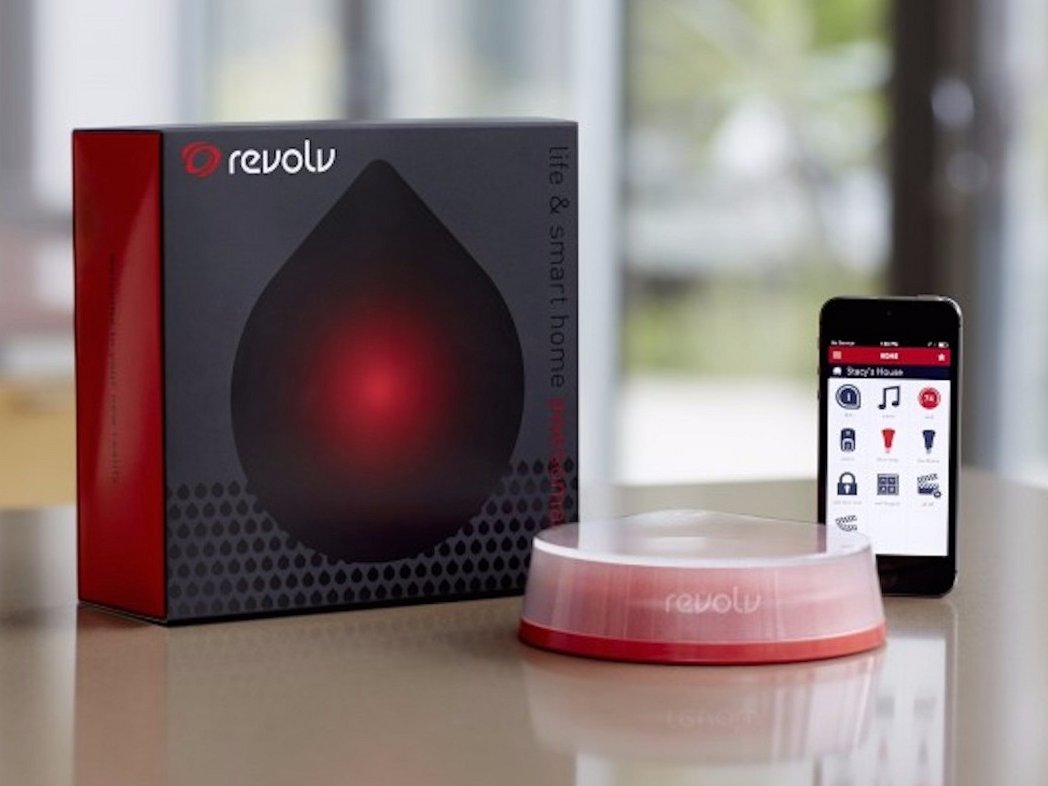
\includegraphics[width=0.8\linewidth]{revolv}
\end{figure}
\end{frame}

\begin{frame}
\frametitle{Mitä jos... joku muu pääsee laitteisiin käsiksi}
\begin{figure}
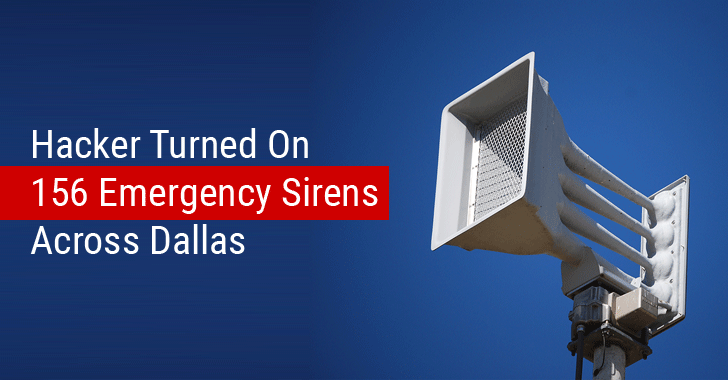
\includegraphics[width=\linewidth]{dallas}
\end{figure}
\end{frame}

\begin{frame}
\frametitle{Mitä jos... joku muu pääsee laitteisiin käsiksi}
\begin{figure}

\includegraphics[width=\linewidth]{burger-king}
\end{figure}
\end{frame}

\section{Välilliset ongelmat}

\begin{frame}
\frametitle{Tietoturva}
\Huge{Jokainen laite Internetissä on potentiaalinen hyökkäyksen väline}
\end{frame}

\begin{frame}
\frametitle{Tietoturva}
DDoS DynDns:ää vastaan 16.10.2016
\begin{itemize}
\item Liikennettä n. 100 000 saastuneesta IoT-laitteesta
\item Datavirta luokkaa 600 Gbps
\item DNS on Internetin peruspalvelu \textrightarrow iso osa Internetistä voidaan rampauttaa
\end{itemize}
\end{frame}

%------------------------------------------------

\begin{frame}
\frametitle{Mitä jäi käteen}
\Huge{IoT on keino, ei päämäärä}

\hfill

\Huge{Ota virhetilanteet huomioon}

\hfill

\Huge{Panosta tietoturvaan}
\end{frame}

%----------------------------------------------------------------------------------------

\end{document}